\section{The role of the \texorpdfstring{$\alpha$}{TEXT} coefficient in the intensity function}\label{app:role_alpha_coef}

Here we seek to determine an intuitive approach to the role of the coefficient $\alpha$ in intensity, Eq.~\refeq{eq:intensity_definition}.
The goal of this approach is to determine a function that will allow to initialize the $\alpha$ parameter for the EM algorithm, for the \textit{smart init}, as it has been done for the $\mu$ coefficient of the baseline.
The starting point is the Algorithm~\ref{algo:1d_inhomogenous_pp}, which allows us to simulate a non-homogenous Poisson process using a given intensity function.
The coefficient $\alpha$ intervenes at two places in this algorithm: when determining $\Bar{\lambda} = \max_{0 \leq t} \lambda(t)$, and upon acceptance, or not, of the points $s_{m+1}$.

Comme évoqué précédemment (TODO : mettre la ref de l'équation de $\Bar{\lambda}$ adapté à notre modèle), $\Bar{\lambda} = \mu_k + \alpha_{k,p}\kappa_{k,p}\pars{m_{k,p}}$, ainsi, plus le coefficient $\alpha$ est grand, plus l'intensité maximale sur l'intervalle $\intervalleFF{0}{T}$ est élevée.
Pour les points sélectionnés $s_{m+1}$, deux cas sont à considérés : lorsque les points sont sur la baseline et lorsque les points sont sur les supports des différents kernels.
Pour plus de clarté, notons l'ensemble des supports des différents kernels $\mathcal{S}_{p}$ :
\begin{equation}
    \mathcal{S}_{p} \coloneqq \bigcup_{i = 1,\dots,n_p} \intervalleFF{t^{(p)}_i + a}{t^{(p)}_i + b}
\end{equation}

Dans le cas où un point sélectionné $s_{m+1}$ se trouve sur la baseline, \cad $s_{m+1} \in \intervalleFF{0}{T} \setminus \mathcal{S}_{p}$, la probabilité d'accepter ce point est égale à $\lambda\pars{s_{m+1}} / \Bar{\lambda} = \mu_k / \Bar{\lambda}$, et donc diminue lorsque $\alpha$ augmente.
De ce fait, plus $\alpha$ augmente, plus la proportion d'activations se trouvant sur la baseline diminue, et inversement, plus la proportion d'activations se trouvant sur les supports des kernels, \cad se trouvant dans $\mathcal{S}_{p}$ est grande.
Cette relation entre valeur de $\alpha$ et proportion d'activations dans $\mathcal{S}_{p}$ est représentée dans la Figure~\ref{fig:ppt_in_support}, où pour chaque valeur du coefficient $\alpha$, de 0 à 5 avec un pas de 0,1, on calcule en ordonnée ladite proportion de la manière suivante :
\begin{equation}
    p_a \coloneqq \frac{\#\enstq{t\in\mathcal{A}_{k,p}}{t\in\mathcal{S}_{p}}}{\# \mathcal{A}_k}
\end{equation}

\begin{figure}[h!]
    \centering
    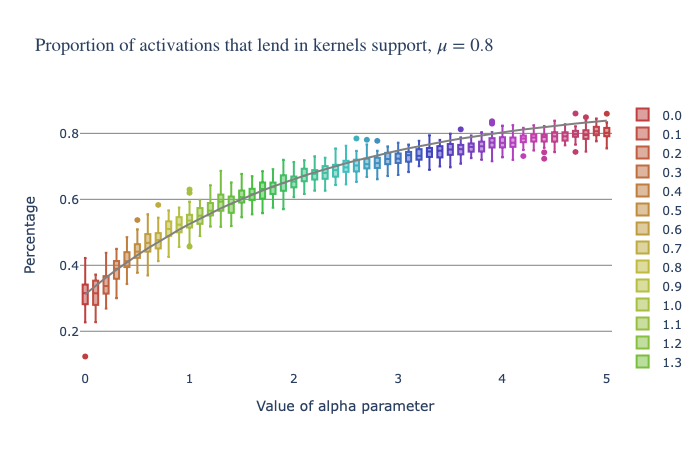
\includegraphics[scale=0.6]{pics/ppt_in_support_transp.png}
    \caption{Proportion des activation générées se trouvant dans $\mathcal{S}$ en fonction du paramètre $\alpha$, où $\mu=0.8, T=180, n_p=73, \intervalleFF{a}{b}=\bracks{30, 800} \times \num{e-3}$, avec 50 simulations pour chaque valeur de $\alpha$. En noir la fonction $f^{-1}(p_a)$}
    \label{fig:ppt_in_support}
\end{figure}

Comme mentionné au préalable, on cherche une fonction, qui, à partir des données, nous permettrait d'avoir une première estimation de $\alpha$, de façon à initialiser l'algorithme EM de façon intuitive.
Une première observation que l'on peut faire à l'aide de cette figure et qu'il existe très probablement une relation entre la valeur du coefficient $\alpha$ et $p_a$.
Si on arrive à établir une telle relation, alors, en prenant son inverse, on sera capable de déterminer une première valeur de $\alpha$ à partir de la proportion $p_a$, qui peut être calculée immédiatement à partir des données.
On pourra alors initier $\alpha$ de la manière suivante :
\begin{equation}
    \alpha^{(0)} = f(p_a)
\end{equation}

Une première observation que l'on peut faire d'emblée, est que, quelques soient les valeurs des hyper-paramètres, $\alpha$, $\mu$, $T$, etc., $p_a$ sera toujours en dessous de 1, par définition.
Ainsi, au vue de la forme de la relation dans la Figure~\ref{fig:ppt_in_support}, une première idée est la suivante :
\begin{equation}\label{eq:alpha_init_1}
    f(p_a) = -\ln \pars{1-p_a}
\end{equation}

Lorsque $\alpha = 0$, l'intensité est réduite à sa baseline, $\lambda_{k,p}(t) = \mu_k, \forall t \in \intervalleFF{0}{T}$, la proportion d'acceptation dans l'algorithme de simulation vaut donc 1, on se retrouve dans le cas simple d'une simulation d'un processus de Poisson homogène (\cad avec une intensité constante).
Ainsi, la proportion des activations se trouvant dans les supports des différents kernels doit être simplement égale à la proportion que représente l'ensemble des supports dans la durée totale.
On note cette proportion $p_s$ :
\begin{equation}
    p_s \coloneqq \frac{n_p \pars{b-a}}{T}
\end{equation}

En remplaçant par les valeurs numériques utilisées pour la Figure~\ref{fig:ppt_in_support}, on obtient bien que $p_s = 0.31$, ce qui est en accord avec la médiane obtenue pour $\alpha = 0$.

Ainsi, une deuxième observation que l'on peut faire est que, si $\alpha$ est toujours positif, alors $p_a$ est toujours plus élevée que $p_s$.
On modifie alors \ref{eq:alpha_init_1} en conséquence :
\begin{equation}
    f(p_a) = -\ln\pars{1-p_a} + \ln\pars{1-p_s} = -\ln\pars{\frac{1 - p_a}{1 - p_s}}
\end{equation}

De plus, plus la baseline est forte, moins $p_a$ augmente rapidement, on veut donc que la courbure diminue lorsque $\mu$ augmente :
\begin{equation}
    f(p_a) = - e^{\mu} \ln\pars{\frac{1 - p_a}{1 - p_s}}
\end{equation}

De même, plus $\mu$ est élevée, plus il est \guill{difficile} pour $p_a$ d'atteindre la limite de 1.
Or, on ne considère pas des valeurs de $\alpha$ trop grandes, afin de rester réaliste, et ainsi on veut surtout une bonne estimation de $\alpha$ pour des valeurs inférieures à 5.
De ce fait, on se propose d'adapter la limite en fonction de $\mu$ :
\begin{equation}
    f(p_a) = - e^{\mu} \ln\pars{\frac{l(\mu) - p_a}{l(\mu)  - p_s}}
\end{equation}
où $l(\mu)$ est une fonction qui vaut 1 lorsque $\mu = 0$ (dans ce cas toutes les activations se trouvent dans $\mathcal{S}$, $p_a = 1$), et qui tend vers $p_s$ lorsque $\mu$ augmente (car on rappelle que $p_a$ ne peut pas être systématiquement inférieur à $p_s$ pour des valeurs positives de $\alpha$).

Ainsi, on propose :
\begin{equation}
    l(\mu) = \pars{\frac{e^{\mu}-1}{5} + \frac{1}{1-p_s}}^{-1} + p_s
\end{equation}

Afin de tester notre fonction d'initialisation, et montrer qu'elle est meilleure que le hasard, on calcule $\alpha^{(0)} = f(p_a)$, pour différentes valeurs de $\mu$ et de $\alpha$, et ce pour 50 simulations à chaque fois.
On calcule ensuite la RMSE (\textit{Root Mean Square Error}).
Le résultat est présenté en Figure~\ref{fig:heatmap_alpha_init_rmse}.

\begin{figure}[h!]
    \centering
    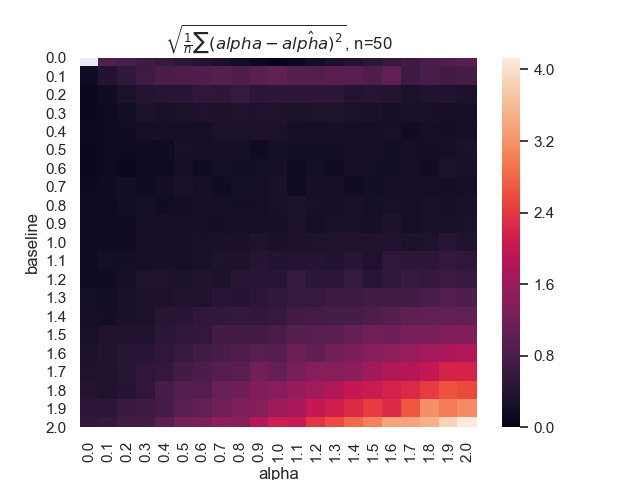
\includegraphics[scale=0.6]{pics/heatmap_baseline_alpha_alpha_init_rmse.jpg}
    \caption{RMSE entre la valeur calculée pour $\alpha^{(0)}$ et sa vraie valeur, pour différentes valeurs de $\mu$ et de $\alpha$}
    \label{fig:heatmap_alpha_init_rmse}
\end{figure}

On observe sur cette figure que l'estimation faite de $\alpha$ est plus que correcte (\cad les cas où la RMSE est plus petite que 1) dans deux situations principales\footnote{On ne prend pas en compte le cas dégénéré où $\mu = \alpha = 0$.} :
\begin{itemize}
    \item lorsque la baseline $\mu$ est faible, mais supérieure à 0,2, et ce pour toutes les valeurs de $\alpha$ ; 
    \item lorsque le coefficient $\alpha$ est faible, et ce pour toutes les valeurs de la baseline.
\end{itemize}

À l'inverse, plus $\mu$ et $\alpha$ augmentent simultanément, moins l'estimation initiale de $\alpha$ est précise.

Il existe un second cas dégénéré, en plus du cas où $\mu = \alpha = 0$ : lorsque $\mu = 0$ et $\alpha > 0$.
Dans ce cas, puisque la baseline est nulle, toutes les activations sont présentent sur les supports des kernels, car en effet, dans l'Algorithme~\ref{algo:1d_inhomogenous_pp}, si $s_{m+1} \notin \mathcal{S}$, alors l'intensité est nulle et donc la probabilité d'accepter un tel point est également nulle.
De ce fait, on a $p_a = 1$, et $l(\mu) = 1$, et alors $f(p_a)$ vaut $+\infty$.
Ainsi, lorsque l'on est dans cette situation, on décide de renvoyer 1 :
\begin{equation}
    f(p_a ; \mu, p_s) = 
    \left\{
		\begin{array}{ll}
			f(p_a) & \mbox{si } \mu > 0 \text{ ou } p_a > 0 \\
			1 & \mbox{sinon}
		\end{array}
	\right.
\end{equation}

\paragraph{Remarque} Dans la pratique, le paramètre $\mu$ de la fonction $f(p_a ; \mu, p_s)$ n'est pas la véritable valeur de la baseline, mais la valeur calculée pour son initialisation, comme définie en [TODO : rajouter ref de l'équation].


